\documentclass[border=5pt]{standalone}
\usepackage[utf8]{inputenc}
\usepackage{amsmath}
\usepackage{amssymb}

\usepackage{tikz}
\usetikzlibrary{shapes.geometric, arrows}

\tikzstyle{startstop} = [rectangle, rounded corners, minimum width=3cm, minimum height=1cm,text centered, draw=black, fill=red!30]
\tikzstyle{io} = [trapezium, trapezium left angle=70, trapezium right angle=110, minimum width=3cm, minimum height=1cm, text centered, draw=black, fill=blue!30]
\tikzstyle{process} = [rectangle, minimum width=3cm, minimum height=1cm, text centered, draw=black, fill=orange!30]
\tikzstyle{decision} = [diamond, minimum width=3cm, minimum height=1cm, text centered, draw=black, fill=green!30]
\tikzstyle{arrow} = [thick,->,>=stealth, rounded corners]
\tikzstyle{fdot} = [circle, minimum width=4pt, fill]
\tikzstyle{line} = [thick,>=stealth, rounded corners]

\begin{document}

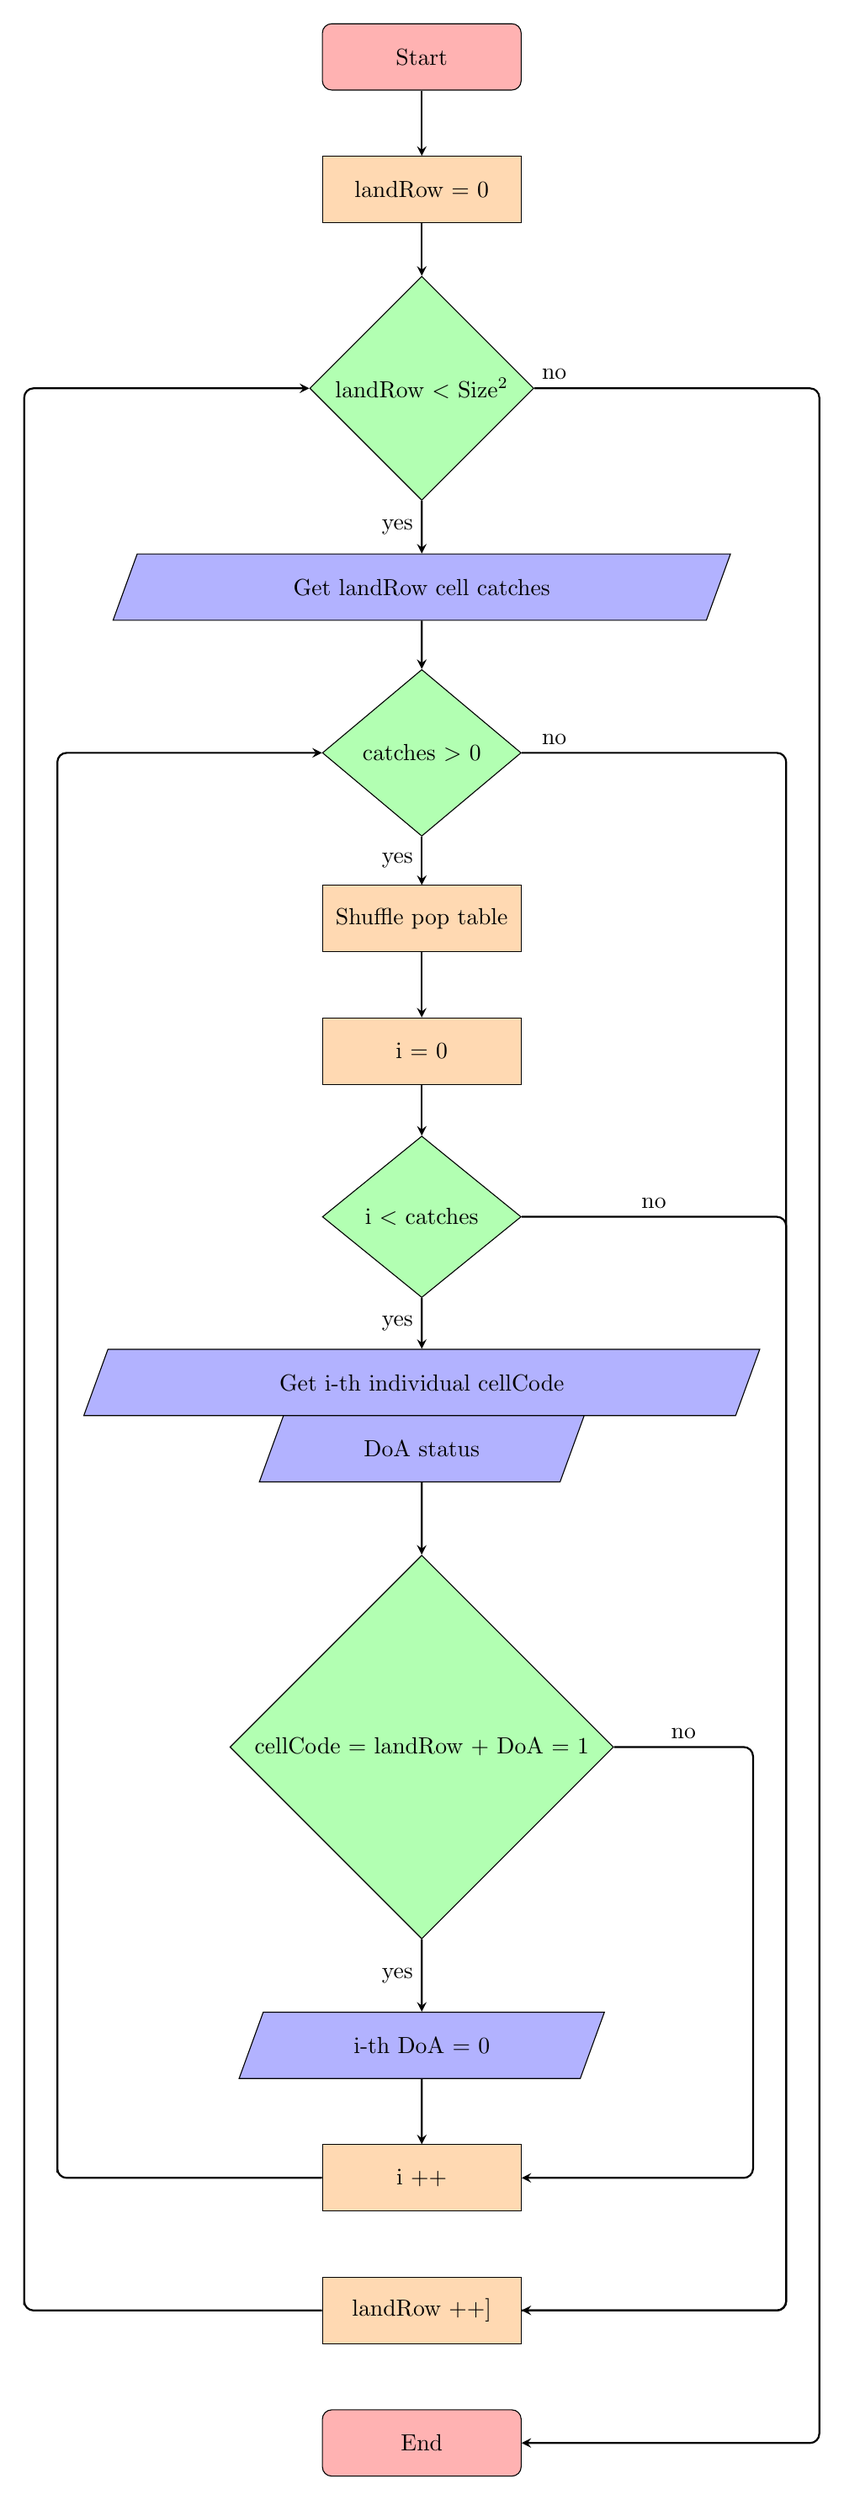
\begin{tikzpicture}[node distance=3cm]

\node (start) [startstop] {Start};
\node (pro1) [process, below of=start, yshift=1cm] {landRow = 0};
\node (dec1) [decision, below of=pro1] {landRow $<$ Size$^2$};
\node (in1) [io, below of=dec1] {Get landRow cell catches};
\node (dec2) [decision, below of=in1, yshift=0.5cm] {catches $>$ 0};
\node (pro2) [process, below of=dec2, yshift=0.5cm] {Shuffle pop table};
\node (pro3) [process, below of=pro2, yshift=1cm] {i = 0};
\node (dec3) [decision, below of=pro3, yshift=0.5cm] {i $<$ catches};
\node (in2) [io, below of=dec3, yshift=0.5cm] {Get i-th individual cellCode};
\node (in3) [io, below of=in2, yshift=2cm] {DoA status};
\node (dec4) [decision, below of=in3, yshift=-1.5cm] {cellCode = landRow + DoA $=$ 1};
\node (out1) [io, below of=dec4, yshift=-1.5cm] {i-th DoA $=$ 0};
\node (pro4) [process, below of=out1, yshift=1cm] {i ++};
\node (pro5) [process, below of=pro4, yshift=1cm] {landRow ++]};
\node (stop) [startstop, below of=pro5, yshift=1cm] {End};

\draw [arrow] (start) -- (pro1);
\draw [arrow] (pro1) -- (dec1);
\draw [arrow] (dec1) -- node[anchor=east] {yes} (in1);
\draw [arrow] (dec1) -| node[anchor=south, xshift=-4cm] {no} + (6,-0.5) |- (stop);
\draw [arrow] (in1) -- (dec2);
\draw [arrow] (dec2) -- node[anchor=east] {yes} (pro2);
\draw [line] (dec2) -| node[anchor=south, xshift=-3.5cm] {no} + (5.5,-0.5) |- (pro5);
\draw [arrow] (pro2) -- (pro3);
\draw [arrow] (pro3) -- (dec3);
\draw [arrow] (dec3) -- node[anchor=east] {yes} (in2);
\draw [arrow] (dec3) -- node[anchor=south, xshift=0cm] {no} + (5.5,0) |- (pro5);
\draw [arrow] (in3) -- (dec4);
\draw [arrow] (dec4) -- node[anchor=east] {yes} (out1);
\draw [arrow] (dec4) -- node[anchor=south, xshift=0cm] {no} + (5,0) |- (pro4);
\draw [arrow] (out1) -- (pro4);
\draw [arrow] (pro4) -| + (-5.5,0) |- (dec2);
\draw [arrow] (pro5) -| + (-6,0) |- (dec1);

\end{tikzpicture}

\end{document}